\documentclass[conference]{IEEEtran}
\IEEEoverridecommandlockouts

\usepackage{cite}
\usepackage{amsmath,amssymb,amsfonts}
\usepackage{algorithm}
\usepackage{algorithmic}
\usepackage{graphicx}
\usepackage{textcomp}
\usepackage[table]{xcolor}
\usepackage{multirow}
\usepackage{booktabs}
\usepackage{url}
\usepackage{float}
\usepackage[T1]{fontenc}
\usepackage{tikz}
\usepackage{pgfplots}
\usetikzlibrary{shapes.geometric,arrows,positioning}
\pgfplotsset{compat=1.18}

\def\BibTeX{{\rm B\kern-.05em{\sc i\kern-.025em b}\kern-.08em
    T\kern-.1667em\lower.7ex\hbox{E}\kern-.125emX}}

\begin{document}

\title{Smart Bus Accident \& Passenger Health Monitoring System\\
Public Transport Emergency Intelligence with Edge AI}

\author{%
    \IEEEauthorblockN{Tanguturi Sharani}
    \IEEEauthorblockA{\textit{School of Electronics Engineering}\\
    \textit{Vellore Institute of Technology}\\
    Chennai, India\\
    22MIS1154@vitstudent.ac.in}
    \and
    \IEEEauthorblockN{Kakarala Sreevallabh}
    \IEEEauthorblockA{\textit{School of Computer Science}\\
    \textit{Vellore Institute of Technology}\\
    Chennai, India\\
    sreevallabh.2022@vitstudent.ac.in}%
}

\maketitle

\begin{abstract}
Conventional public transport emergency systems focus primarily on vehicle-level indicators such as accident location and impact severity, with little visibility into the real-time physiological condition of passengers.
This work presents a Smart Bus Accident \& Passenger Health Monitoring System that unifies bus-mounted IoT sensing, wearable-derived vital signs, edge intelligence, and cloud-assisted analytics to enable human-aware emergency response.
In our prototype, accident and health data are acquired from an ESP32-based accident detection unit and smartwatch-inspired passenger signals, then replayed via curated CSV datasets into a Flutter application.
Passenger-wise severity is inferred using Google's Gemini generative AI API instead of a local LLM, yielding Normal, Panic, or Critical classifications accompanied by structured triage summaries.
Interactive analytics dashboards visualize impact profiles, heart-rate trajectories, and severity distributions, illustrating how low-cost edge intelligence can transform post-accident decision making without expensive hardware.
\end{abstract}

\begin{IEEEkeywords}
smart transportation, edge intelligence, emergency response, wearable sensing, ESP32, Gemini API, human-aware IoT
\end{IEEEkeywords}

\section{Introduction}

Public bus systems transport millions of commuters daily in dense urban environments.
When severe accidents occur, current emergency workflows are triggered by coarse vehicle-level information such as GPS location, impact detection, and driver phone calls.
First responders arrive with only a vague understanding of how many passengers are injured, which individuals require immediate life-saving intervention, and who is merely in panic but physiologically stable.

The absence of passenger-specific physiological insight leads to generalized, non-prioritized medical care, wasting the critical ``golden hour'' after trauma.
On the other hand, equipping every passenger with certified medical devices or high-end communication infrastructure is economically infeasible for most public operators.
There is therefore a strong need for a system that leverages affordable IoT components, commodity wearables, and modern AI models to generate fine-grained, privacy-preserving emergency intelligence.

This paper proposes a practical architecture for a Smart Bus Accident \& Passenger Health Monitoring System, implemented as an academic prototype.
The system integrates an ESP32-based accident detection unit, wearable-like passenger health data, a Flutter mobile and admin dashboard, and a cloud-based large language model (LLM) accessed via API to reason about multi-sensor time series.
Unlike traditional threshold-based alarm systems, our approach produces structured, passenger-wise summaries that aid triage while still remaining deployable on low-cost hardware.

\section{System Overview}

\subsection{Four-Layer Architecture}

The proposed system follows a four-layer design derived from transportation safety requirements:

\begin{enumerate}
    \item \textbf{Bus Accident Detection Layer}: An ESP32 microcontroller with an IMU, alcohol sensor, and SOS button continuously monitors crash, rollover, and hazardous driving conditions.
    \item \textbf{Passenger Health Monitoring Layer}: Each passenger is associated with a wearable device (e.g., smartwatch) that measures heart rate, heart-rate variability (HRV), motion intensity, and blood oxygen saturation (SpO\textsubscript{2}).
    \item \textbf{Local Intelligence \& Gateway Layer}: A gateway device (smartphone or bus tablet) aggregates accident and health data and forwards compact summaries to a cloud-hosted LLM through an HTTPS API.
    \item \textbf{Emergency Response Layer}: Passenger-wise severity maps, synthesized by the LLM, are presented on an operator console and can be forwarded to emergency dispatch services.
\end{enumerate}

\subsection{Implemented Prototype}

In the academic prototype presented here, raw sensor streams are emulated using curated CSV files that reflect realistic accident and health trajectories.
These files are ingested by a Flutter application which implements:

\begin{itemize}
    \item Passenger login and seat registration,
    \item Setup screen for data loading and API-key configuration,
    \item Passenger dashboard and detailed vital view,
    \item Emergency alert interface,
    \item Administrator bus overview, and
    \item Analytics dashboard with time-series plots and severity distributions.
\end{itemize}

The core idea is to preserve the complete data and control flow of the final field system while avoiding the complexity of live sensor integration during the course project phase.

\section{Hardware and Connectivity}

\subsection{Bus Accident Detection Unit}

The accident detection unit is built around an ESP32 DevKit V1 microcontroller.
Table~\ref{tab:hardware} lists the primary components and their roles.

\begin{table}[!t]
    \caption{Bus Accident Detection Unit Components}
    \label{tab:hardware}
    \raggedright
    \scriptsize
    \begin{tabular}{llp{3.4cm}}
        \toprule
        \textbf{Component} & \textbf{Interface} & \textbf{Function} \\
        \midrule
        ESP32 DevKit V1 & -- & Central controller, BLE gateway, Wi-Fi client \\
        MPU6050 IMU & I\textsuperscript{2}C (GPIO 21/22) & Measures acceleration and angular velocity to detect collision, rollover, and sharp braking events \\
        MQ-3 Alcohol Sensor & Analog (GPIO 34) & Monitors driver breath alcohol concentration and raises alerts for unsafe driving \\
        SOS Push Button & GPIO 15 (INPUT\_PULLUP) & Manual emergency trigger from driver or conductor \\
        Power Supply & Bus battery + regulator & Provides stable 3.3\,V/5\,V rails for all sensors \\
        \bottomrule
    \end{tabular}
\end{table}

The ESP32 periodically aggregates IMU features (acceleration magnitude, gyroscope magnitude) and contextual flags (alcohol threshold crossing, SOS activation).
In a full deployment these features would be packaged into BLE or Wi-Fi messages and sent to the gateway device.
In our implementation, equivalent time-series values are exported into \texttt{bus\_sensor\_data.csv} and replayed by the application.

\subsection{Passenger Health Monitoring}

Passenger physiology is modeled after data streams typically available from consumer smartwatches.
For each seat, the following pseudo-sensor fields are logged in \texttt{passenger\_health\_data.csv}:

\begin{itemize}
    \item Heart rate (beats per minute),
    \item Heart-rate variability (milliseconds),
    \item Motion intensity (normalized activity index),
    \item Skin temperature (degrees Celsius), and
    \item SpO\textsubscript{2} (percentage).
\end{itemize}

The dataset captures both stable baseline segments and abrupt changes at the moment of collision.
For example, a passenger with pre-existing cardiac disease shows a sharp heart-rate spike and HRV collapse, whereas a passenger with hypertension exhibits bradycardia and SpO\textsubscript{2} drop due to shock.

\subsection{Connectivity Model}

The envisioned connectivity model is:

\begin{enumerate}
    \item Smartwatch $\rightarrow$ smartphone via Bluetooth Low Energy (BLE),
    \item ESP32 bus unit $\rightarrow$ gateway via BLE, and
    \item Gateway $\rightarrow$ cloud LLM backend via Wi-Fi or cellular network.
\end{enumerate}

Only compact, privacy-preserving summaries and severity labels are forwarded to emergency services; raw physiological traces remain local to the gateway.

\section{Edge Intelligence with Gemini API}

\subsection{Motivation for Cloud-Hosted LLM}

Early design options considered deploying a local LLM directly on the gateway device.
Although this maximizes privacy and offline robustness, it imposes high memory and compute requirements on smartphones and tablets.
For an academic prototype with limited edge resources, we replace the local LLM with Google's Gemini model accessed through a REST API, while preserving the same reasoning behavior and data structures.

\subsection{Data Aggregation and Prompt Construction}

The Flutter application parses the two CSV files and derives per-passenger baseline and latest readings.
For each passenger $i$, the system constructs a compact textual summary:
\begin{align}
    \mathbf{s}_i = [&\text{seat}, \text{ID}, \text{name}, \nonumber \\
    &\text{baseline HR/HRV}, \text{current HR/HRV}, \nonumber \\
    &\text{motion change}, \text{SpO}_2, \text{comorbidities}], \nonumber
\end{align}
and combines these with global accident descriptors such as collision time and peak acceleration.

The full prompt instructs the model to classify each passenger into \emph{Normal}, \emph{Panic}, or \emph{Critical} and to respond strictly in JSON format with a list of assessments and an overall emergency summary.
The back-end enforces \texttt{responseMimeType = application/json} to avoid natural-language outputs that would require brittle parsing.

\subsection{Structured Output and Triage Map}

Gemini responds with an object of the form
\begin{equation}
    \{\texttt{assessments}, \texttt{emergency\_summary}, \texttt{recommended\_priority}\},
\end{equation}
where each item in \texttt{assessments} carries seat number, passenger ID, status label, and one-sentence reasoning.
The application maps these into strongly typed Dart classes and overlays them on the bus seat layout.
An example output sentence is:
\emph{``Seat A03 (heart condition): Critical --- HR 68$\rightarrow$142\,bpm, HRV collapse, almost no motion, SpO$_2$ 89\%, high risk of decompensation.''}

\begin{figure}[!t]
    \raggedright
    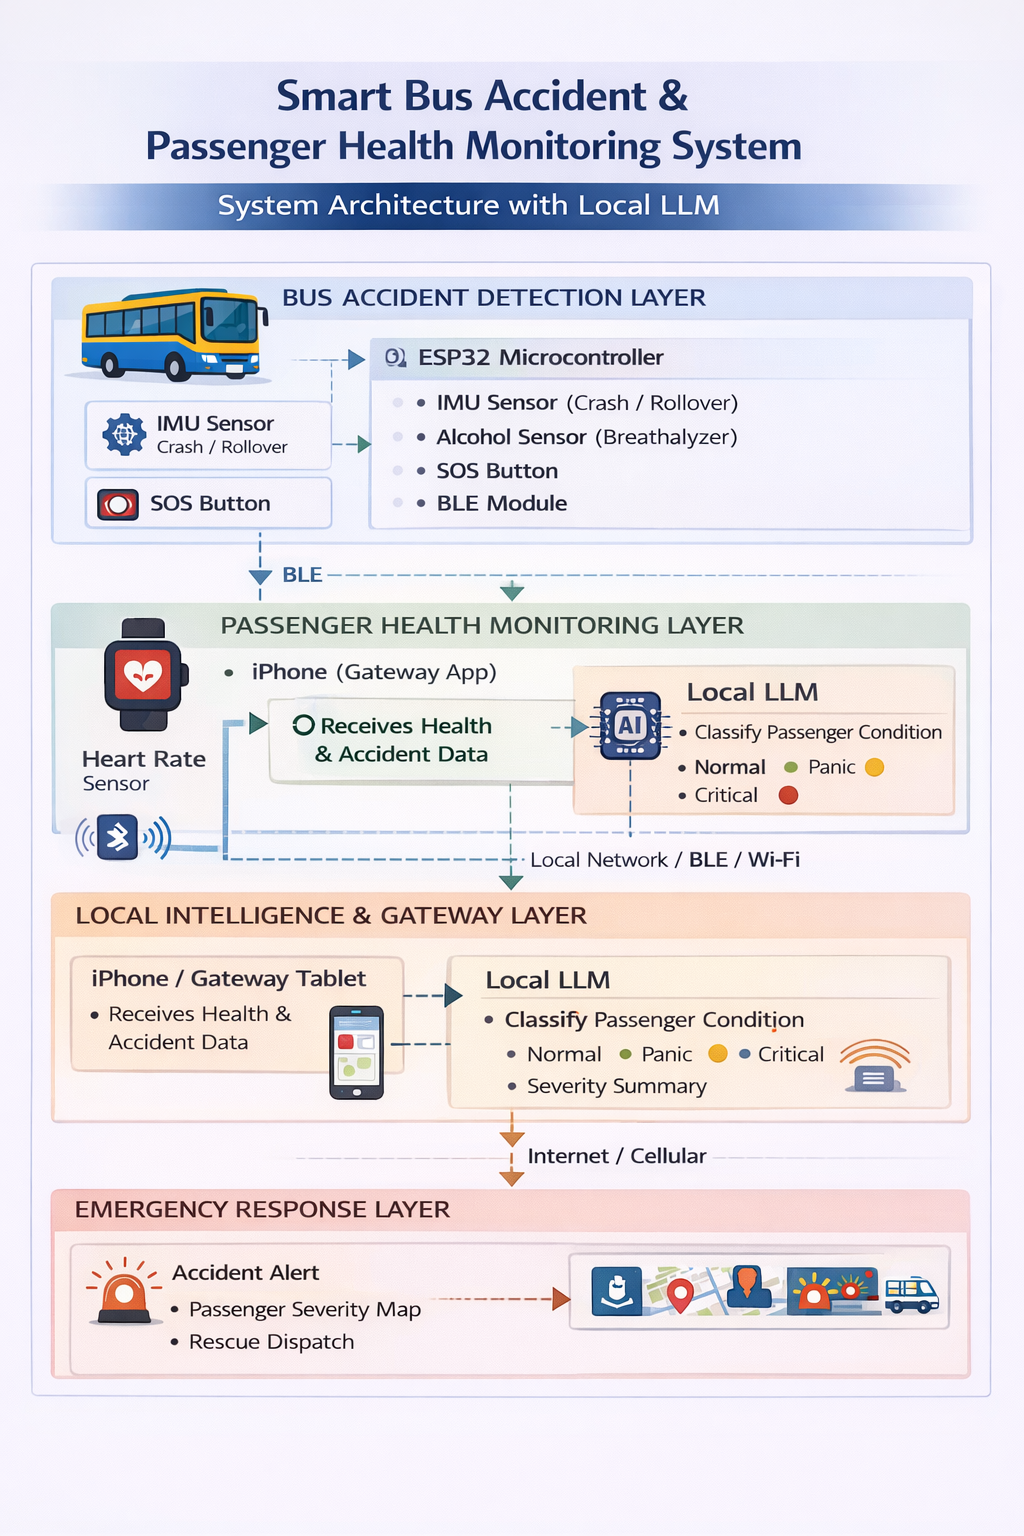
\includegraphics[width=0.95\linewidth]{Architecture (4).png}
    \caption{High-level system architecture of the Smart Bus Accident \& Passenger Health Monitoring System.
    The bus accident detection layer, passenger health monitoring layer, local intelligence \& gateway layer, and emergency response layer form a pipeline from raw sensor signals to passenger-wise severity reports.}
    \label{fig:architecture_bus}
\end{figure}

\section{Analytics and Visualization}

Beyond binary alerts, operators require an interpretable overview of how the accident unfolded and how different passenger groups reacted.
The Flutter application therefore includes a dedicated analytics screen powered by time-series plotting libraries.

\subsection{Bus Dynamics}

Acceleration magnitude and speed over time are visualized as smoothed line charts.
Normal driving is characterized by minor oscillations around $9.8$\,m/s\textsuperscript{2}; the simulated collision appears as a prominent spike followed by a plateau at zero speed.
This contextualizes the severity and duration of the impact for investigators and insurance analysis.

\subsection{Passenger Vital Trends}

For each passenger, heart rate and HRV traces are normalized against their own baseline to avoid misleading comparisons across individuals.
The analytics view overlays multiple colored curves, one per passenger, revealing heterogeneous physiological trajectories: some show short-term panic responses, while others enter potentially life-threatening instability.

\subsection{Severity Distribution}

Once Gemini assessments are available, the system computes counts of Normal, Panic, and Critical passengers and renders both bar and pie charts.
These distributions help emergency coordinators estimate how many advanced life support teams and ambulances should be dispatched.

\section{Discussion}

\subsection{Benefits}

The prototype demonstrates that even when sensor readings are replayed from CSV logs, the complete processing chain from raw measurements to triage guidance can be validated end-to-end.
The combination of hand-crafted features, LLM-based reasoning, and intuitive visualization offers:

\begin{itemize}
    \item \textbf{Human-centric response}: Focus shifts from vehicle damage to passenger health.
    \item \textbf{Low hardware cost}: ESP32, IMU, and commodity wearables are affordable and widely available.
    \item \textbf{Incremental deployment}: Operators may start with offline analytics and graduate to live integration as infrastructure matures.
\end{itemize}

\subsection{Limitations}

Reliance on a cloud-hosted LLM introduces latency and requires network connectivity at the time of accident.
The present CSV datasets, while realistic, cover only a limited set of scenarios and medical profiles.
Furthermore, the model supplies decision support rather than clinical diagnoses; human experts remain responsible for final judgments.

\section{Conclusion and Future Work}

This paper presented an integrated architecture for a Smart Bus Accident \& Passenger Health Monitoring System and its implementation as a Flutter-based academic prototype.
By combining ESP32-class IoT measurements, wearable-inspired passenger vitals, structured CSV datasets, Gemini-based triage analysis, and rich analytics dashboards, the system illustrates a feasible pathway toward human-aware public transport safety.

Future work will focus on (i) replacing CSV replays with live BLE and Wi-Fi integrations, (ii) experimenting with lightweight on-device models to reduce dependence on cloud APIs, and (iii) expanding the dataset to cover a broader range of accident severities and passenger demographics.

\section*{Acknowledgment}

The authors thank the course instructor and teaching staff of ECE3502 \textit{IoT Domain Analyst} for guidance in shaping the system requirements and evaluation metrics.

\begin{thebibliography}{00}
\bibitem{who_golden_hour}
World Health Organization, ``Emergency care systems for universal health coverage: ensuring timely care for the acutely ill and injured,'' 2018.

\bibitem{esp32}
Espressif Systems, ``ESP32 Series: Datasheet,'' v3.9, 2023. [Online]. Available: \url{https://www.espressif.com/}

\bibitem{smart_wearables}
P. Bonato, ``Wearable sensors and systems,'' \textit{IEEE Engineering in Medicine and Biology Magazine}, vol. 29, no. 3, pp. 25--36, 2010.

\bibitem{gemini}
Google, ``Gemini API: Overview and documentation,'' 2025. [Online]. Available: \url{https://ai.google.dev/}
\end{thebibliography}

\end{document}
